%*****************************************************************************
%  CHAPTER 4: RESULTS AND DISCUSSION
%
%  STATUS AS OF 11 NOVEMBER 2026: PARTIAL.
%
%  Everything stated below is drawn from data that exists in the repository
%  today. Nothing is estimated, projected or invented.
%
%  The sections marked \pending{} are the ones that cannot be written until
%  run 2 is harvested. They are laid out in full so the numbers drop straight
%  in. DO NOT fill them with placeholder values: an empty table that says
%  "collection in progress" is defensible, a table of invented numbers is not.
%
%  Data sources, all in the THESIS repository:
%    DATA/thesis/growth_dataset.csv                    (D1-D12, 90 rows)
%    DELIVERABLES/D1_calibration_and_irrigation/       (irrigation, soil moisture)
%    DELIVERABLES/D7_reliability/                      (power, faults, summary)
%    DELIVERABLES/D7_reliability/vision/               (GPR validation, ROI, glare)
%*****************************************************************************

\chapter{Results and Discussion}
\label{chap:results}

\ifpdf
    \graphicspath{{Chapter4/Figs/Raster/}{Chapter4/Figs/PDF/}{Chapter4/Figs/}}
\else
    \graphicspath{{Chapter4/Figs/Vector/}{Chapter4/Figs/}}
\fi

% A visible marker for work still in progress. Delete the macro and every
% \pending{...} call once the chapter is complete.
\newcommand{\pending}[1]{%
  \par\medskip\noindent\fbox{\parbox{0.96\linewidth}{\footnotesize\textbf{Data
  collection in progress.} #1}}\par\medskip}

This chapter reports the results obtained from the deployed system. The data
presented here were collected during the second instrumented grow-out, sown on
29 October 2026, and cover days 1 to 12 of a 30-day cycle. Results that depend
on the harvest are identified as such and are not yet available.

%=============================================================================
\section{Dataset Completeness}
%=============================================================================

The capture schedule calls for one record per pot per day, or nine rows per
day. Table~\ref{tab:completeness} summarises what was obtained.

\begin{table}[ht]
\centering
\caption{Dataset completeness for the second grow-out, days 1 to 12}
\label{tab:completeness}
\begin{tabular}{lr}
\toprule
\textbf{Quantity} & \textbf{Value} \\
\midrule
Sowing date                       & 29 October 2026 \\
Cycle length                      & 30 days \\
Days elapsed at time of writing   & 12 \\
Capture days due                  & 12 \\
Capture days recorded             & 10 \\
Rows due                          & 108 \\
Rows written                      & 90 \\
Completeness                      & 83.3\,\% \\
Rows with usable soil moisture    & 90 \\
Rows with missing soil moisture   & 0 \\
Rows carrying an anomaly flag     & 0 \\
\bottomrule
\end{tabular}
\end{table}

Two capture days, D2 and D3, were not recorded. The cause was loss of mains
power to the controller before the scheduled noon capture, and the days were
entered in the field log as missed rather than back-filled from a later frame.
A missed day is an unrecoverable gap in the series: the capture is tied to a
fixed solar time, so a frame taken at any other hour is not comparable. No
value was interpolated into those rows. This decision is recorded here because
it bears on every subsequent analysis: the growth series for this run has ten
observations per pot, not twelve.

%=============================================================================
\section{Growing Environment and Treatment Adherence}
%=============================================================================

\subsection{Germination Phase}

The controller holds every pot at the germination band of 50 to 60\,\%
volumetric water content until the treatment bands are enabled. For this run,
germination mode ran from 29 October to 5 November, and the treatment bands
were switched on at D8.

Adherence during germination was poor. Across 160 snapshots per pot, only P-02
and P-03 entered the 50 to 60\,\% band at all, for 41.2\,\% and 15.0\,\% of
samples respectively. The remaining seven pots never entered the band during
germination. In every case the deviation was upward: the medium was prepared
moist and the pots began the run well above the target, so the controller had
no action available to it. The dose-and-wait rule can add water but cannot
remove it, and the pots could only approach the band by evaporative loss.

\subsection{Treatment Phase}

Table~\ref{tab:sm_by_group} gives the group mean soil moisture for each
recorded day.

\begin{table}[ht]
\centering
\caption{Group mean soil moisture by day, in per cent volumetric water
content. Treatment bands were enabled at D8.}
\label{tab:sm_by_group}
\begin{tabular}{lrrr}
\toprule
\textbf{Day} & \textbf{Low (30--40\,\%)} & \textbf{Optimal (50--60\,\%)} & \textbf{High (70--80\,\%)} \\
\midrule
D1  & 59.8 & 84.3 & 98.1 \\
D4  & 68.5 & 88.8 & 99.0 \\
D5  & 69.1 & 87.6 & 98.1 \\
D6  & 61.2 & 85.3 & 95.5 \\
D7  & 65.3 & 83.3 & 95.7 \\
D8  & 71.5 & 72.0 & 89.0 \\
D9  & 65.4 & 69.2 & 90.3 \\
D10 & 61.8 & 67.7 & 89.0 \\
D11 & 75.1 & 67.7 & 89.0 \\
D12 & 61.4 & 53.9 & 78.6 \\
\bottomrule
\end{tabular}
\end{table}

Three observations follow directly from the table, and all three are
unfavourable to the experiment as it currently stands.

First, no group is inside its assigned band. At D12 the low group sits at
61.4\,\% against a target of 30 to 40\,\%, the optimal group at 53.9\,\%
against 50 to 60\,\%, and the high group at 78.6\,\% against 70 to 80\,\%.
Only the optimal and high groups are within their bands at all, and only on
the most recent day.

Second, the groups are ordered correctly but not separated adequately. The
low group is consistently drier than the optimal group, and the optimal group
drier than the high group, which is the required ordering. The separation
between low and optimal, however, is 7.5 percentage points at D12, where the
design calls for a gap of at least 10 and preferably 20 points.

Third, the pots are drying rather than being driven to their targets. Across the
whole run only three irrigation events fired, delivering 51\,mL in total
across the whole array. The low group is approaching its band from above by
evaporation alone, and the rate of that approach is set by the weather, not by
the controller.

The consequence for the study is stated plainly. The soil moisture term in the
yield model is only meaningful if the treatments produce genuinely different
water regimes. At present they do not, and if the run finishes in this state
the model will be fitted across a narrow and partly overlapping range of soil
moisture, which limits what can be claimed from it. This is recorded here as a
result, not deferred to the limitations section.

\subsection{Irrigation Events}

Table~\ref{tab:irrigation} lists every irrigation event delivered in this run.

\begin{table}[ht]
\centering
\caption{Irrigation events delivered during the second grow-out}
\label{tab:irrigation}
\begin{tabular}{llrrr}
\toprule
\textbf{Timestamp} & \textbf{Pot} & \textbf{Phase} & \textbf{VWC before} & \textbf{Dose (mL)} \\
\midrule
2026-11-05 11:25 & P-02 & Germination & 49.9 & 16.2 \\
2026-11-06 09:35 & P-05 & Optimal     & 50.0 & 16.0 \\
2026-11-07 10:06 & P-05 & Optimal     & 49.1 & 18.8 \\
\bottomrule
\end{tabular}
\end{table}

All three events targeted 55.0\,\% volumetric water content, delivering
51.0\,mL in total. Each dose was computed from the measured deficit at a rate
of 3.18\,mL per percentage point, and each fired as the pot reached the lower
bound of its band, which is the behaviour the firmware specifies. The
actuation path is therefore demonstrated to work. The small number of events
reflects the pots being above their bands for almost the whole period, not a
failure of the valves or the pump.

%=============================================================================
\section{Canopy Measurement}
%=============================================================================

\subsection{The Measure Used}

The canopy measure reported here is the pot-area Green Pixel Ratio, denoted
\texttt{cell\_gpr}. Each pot is assigned the region of the image whose pixels
lie closer to that pot's centre than to any other pot's centre, bounded at a
radius of 175\,px, which corresponds to approximately 13\,cm at the measured
scale of 1.34\,px\,mm$^{-1}$. The regions do not overlap.

This replaces the fixed circular region of interest described in
Chapter~\ref{chap:methodology} as originally proposed. The reason for the
change is given in Section~\ref{sec:roi_change} below and is itself a result
of the first grow-out.

\subsection{Growth Series}

Table~\ref{tab:gpr_by_group} gives the group mean pot-area GPR by day.

\begin{table}[ht]
\centering
\caption{Group mean pot-area Green Pixel Ratio by day, in per cent of the
pot's measurement area}
\label{tab:gpr_by_group}
\begin{tabular}{lrrr}
\toprule
\textbf{Day} & \textbf{Low} & \textbf{Optimal} & \textbf{High} \\
\midrule
D1  & 0.000 & 0.000 & 0.000 \\
D4  & 0.000 & 0.057 & 0.100 \\
D5  & 0.000 & 0.057 & 0.093 \\
D6  & 0.000 & 0.100 & 0.173 \\
D7  & 0.250 & 0.200 & 0.227 \\
D8  & 0.150 & 0.130 & 0.230 \\
D9  & 0.100 & 0.060 & 0.160 \\
D10 & 0.067 & 0.050 & 0.173 \\
D11 & 0.193 & 0.067 & 0.290 \\
D12 & 0.223 & 0.043 & 0.193 \\
\bottomrule
\end{tabular}
\end{table}

The values are very small. A pot-area GPR of 0.2\,\% corresponds to a canopy
occupying roughly one five-hundredth of the pot's measurement area. At D12 the
plants are seedlings with two to four true leaves, and the series has not yet
entered the phase of rapid canopy expansion on which the yield model depends.

The series is also not yet monotonic. Group means rise to D7 or D8 and then
fluctuate without a clear trend. Two factors contribute. The first is scale:
at a canopy of a few hundred pixels, a difference of fifty pixels between
consecutive days is a visible change in the ratio, so day-to-day noise is
large relative to the signal. The second is illumination: noon irradiance at
the site varies by roughly a factor of seven between a clear and an overcast
day, and although the exposure control normalises mean frame brightness, it
cannot recover saturation in a canopy that is genuinely dimmer.

\pending{The growth series will be extended to D30 as the run completes.
The analysis of canopy expansion rate, and the separation of the growth
curves by treatment group, require the full series and are not attempted on
twelve days of seedling data.}

%=============================================================================
\section{Validation of the Green Pixel Ratio}\label{sec:gpr_validation}
%=============================================================================

The question this section answers is whether the Green Pixel Ratio produced by
the segmentation corresponds to the canopy a human observer would identify. It
is distinct from the calibration procedures of Chapter~\ref{chap:methodology},
which establish that the apparatus works; this section establishes that the
measurement means something.

\subsection{Procedure}

Two annotators, Cedric Tan and Kent Godinez, independently hand-labelled the
leaf blades in eighteen pot images drawn from two noon frames, D12 and D13 of
the first grow-out, captured under the same camera, thresholds and settings
used in the reported run. For each pot the automatic mask was compared against
each manual mask pixel by pixel, yielding true positives, false positives and
false negatives, from which precision, recall, Intersection over Union and the
Dice coefficient were computed. The two manual masks were also compared
against each other to establish how closely two humans agree, which gives the
benchmark against which the algorithm should be judged.

\subsection{Results}

\begin{table}[ht]
\centering
\caption{Agreement between the automatic segmentation and manual annotation,
pooled over 18 pot images}
\label{tab:gpr_validation}
\begin{tabular}{lcccc}
\toprule
 & \textbf{vs Cedric} & \textbf{vs Kent} & \textbf{vs both} & \textbf{Cedric vs Kent} \\
\midrule
Pixel IoU                & 0.64 & 0.64 & 0.64 & 0.79 \\
GPR mean absolute error  & 0.29\,pp & 0.27\,pp & 0.28\,pp & 0.19\,pp \\
GPR bias                 & $-0.05$\,pp & $+0.14$\,pp & $+0.04$\,pp & --- \\
Precision (pooled)       & --- & --- & 0.77 & --- \\
Recall (pooled)          & --- & --- & 0.79 & --- \\
\bottomrule
\end{tabular}
\end{table}

Three findings follow.

The algorithm carries no systematic bias. Its GPR sits between the two
annotators, with a pooled bias of $+0.04$ percentage points against their
average. It is not consistently over-reading or under-reading the canopy.

The algorithm is less precise than a human, but not by an order of magnitude.
Pixel IoU against the humans is 0.64, where the two humans agree with each
other at 0.79. The gap is real and should not be glossed. It reflects
disagreement at leaf boundaries, where a few pixels of soil or shadow are
included or excluded, and these boundary pixels are a large fraction of the
total at the canopy sizes measured.

The human benchmark is itself well short of unity. Two trained annotators
labelling the same leaf blades agree at IoU 0.79, not 0.95. This matters for
how the algorithm's performance should be read: a measure of leaf area from
an overhead image has an irreducible ambiguity at the boundary, and no
segmentation method can be expected to exceed the agreement that humans
achieve among themselves.

Figure~\ref{fig:error_map} shows where the disagreement falls.

\begin{figure}[ht]
\centering
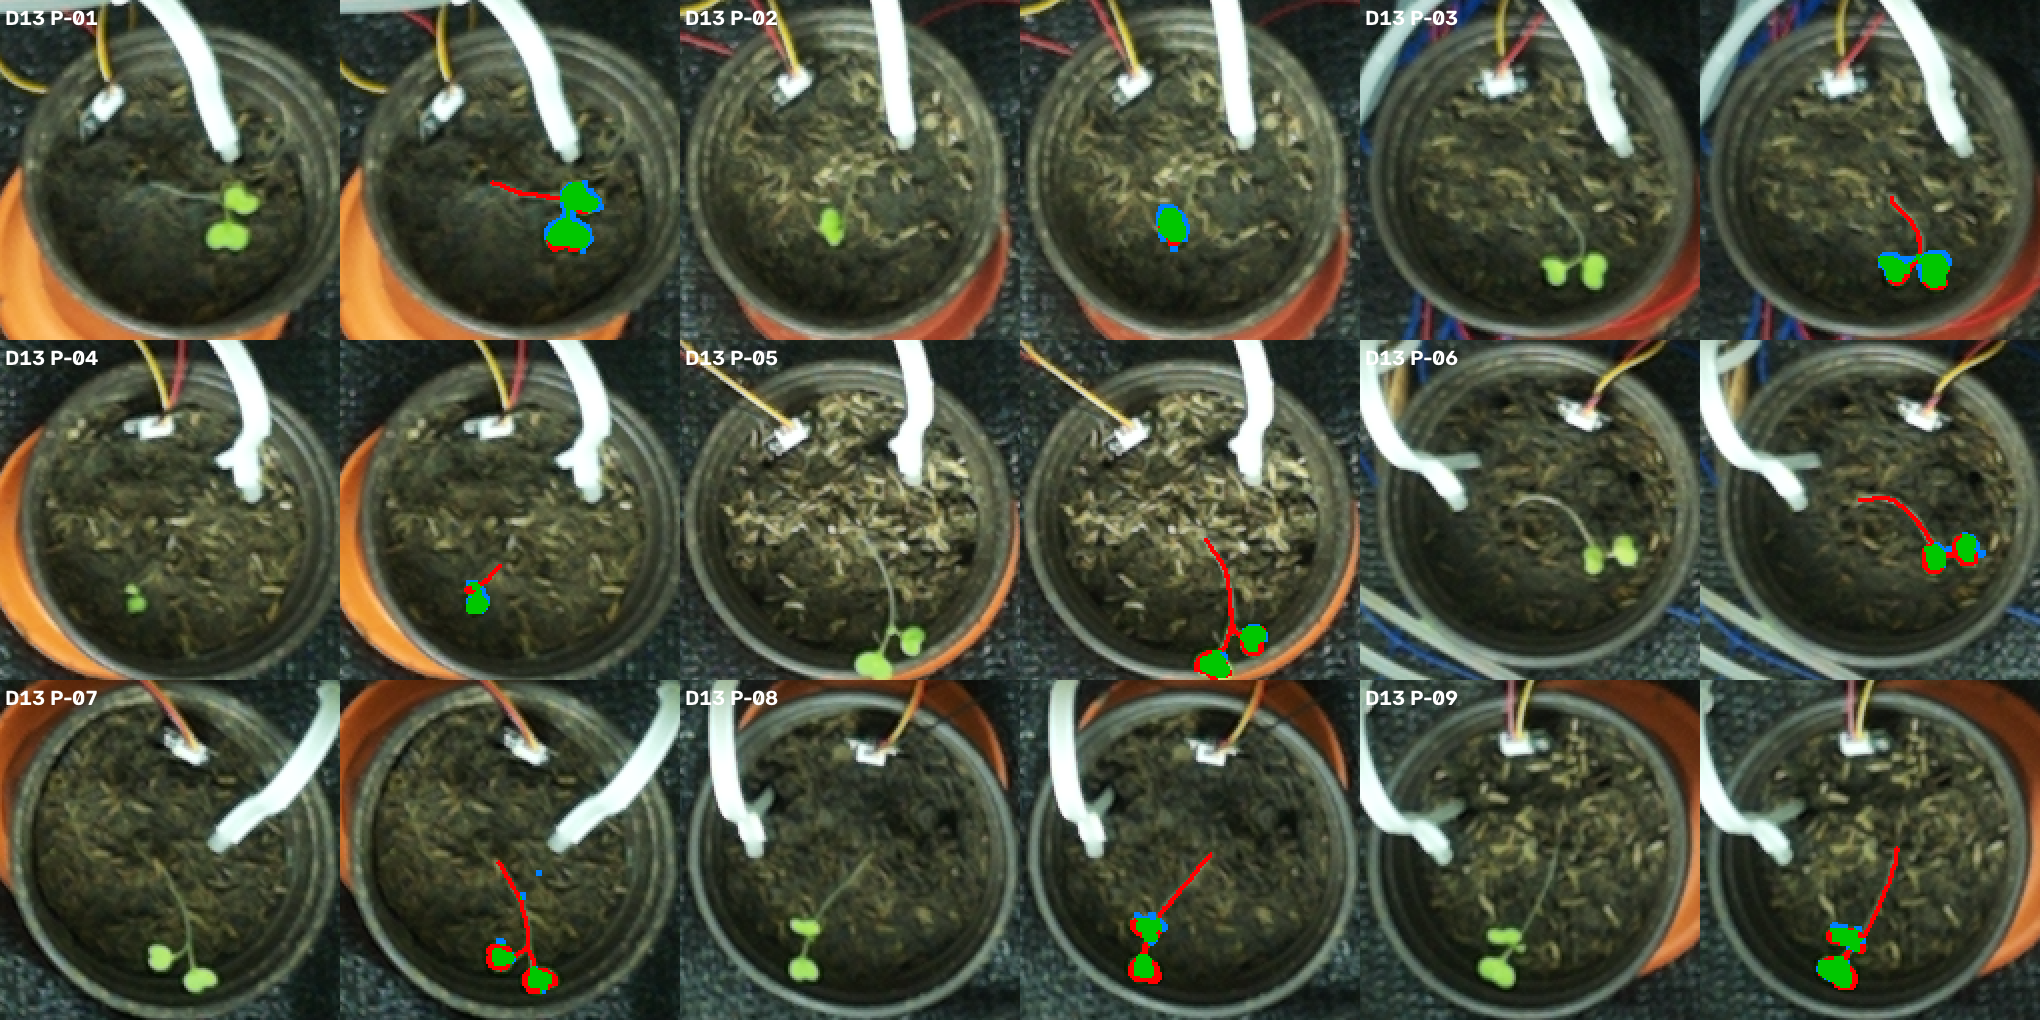
\includegraphics[width=0.8\linewidth]{gpr_error_map_D13.png}
\caption[GPR validation error map]{Spatial distribution of agreement between
the automatic segmentation and manual annotation on the D13 frame. Green
denotes agreement, red denotes canopy missed by the algorithm, and blue
denotes pixels claimed by the algorithm that the annotator did not label.}
\label{fig:error_map}
\end{figure}

The disagreement is concentrated at leaf edges rather than distributed across
leaf interiors, which is consistent with a boundary-definition effect rather
than a threshold that is simply set wrong.

%=============================================================================
\section{Measurement Geometry and Its Stability}\label{sec:roi_change}
%=============================================================================

\subsection{Why the Fixed Circular Region Was Abandoned}

During the first grow-out the canopy measure was computed inside a fixed
circle of 77\,px radius centred on each pot. Plants in that run developed
pronounced phototropic lean, and leaves that extended past the pot rim fell
outside the circle. The circle returned a Green Pixel Ratio of exactly zero
for P-05 and P-07 on six days each, and for P-01 on three days, while those
plants were alive and visibly green in the raw frames.

A measure that reports zero canopy for a living plant is not recording a
small error; it is recording the wrong quantity. The measure was therefore
redefined as the non-overlapping pot area described above, which retains
leaves that lean beyond the rim while still attributing every pixel to exactly
one pot. The redefinition was applied to the retained frames of the first run
and is the measure used throughout the second run.

\subsection{Camera Stability}

Table~\ref{tab:roi_drift} records the measured displacement of the camera
against the run reference frame.

\begin{table}[ht]
\centering
\caption{Camera displacement measured against the reference frame}
\label{tab:roi_drift}
\begin{tabular}{llp{0.45\linewidth}}
\toprule
\textbf{Day} & \textbf{Shift} & \textbf{Action taken} \\
\midrule
D1 & Pots and camera repositioned during setup & Regions fitted three times, at 13:15, 14:38 and 14:45; each fit logged with a backup of the previous file \\
D4 & 7 to 8\,px & None required \\
D5 & 5\,px & None required \\
D6 & 16\,px right & Regions re-centred at 16:00, applying from D7; previous file retained \\
D7 & 1\,px from D6 & None required \\
D11 & Reference re-based on the D11 frame & Circles moved $-21$, $+12$\,px; each capture now matched against the D11 reference before writing \\
\bottomrule
\end{tabular}
\end{table}

The 16\,px displacement at D6 did not corrupt the measurements for D4 to D6.
The reported measure counts each pot's whole area out to 175\,px, and a
displacement of 16\,px leaves every pot well inside its own area, so the
canopy pixels continued to be attributed to the correct pot. This is a
property of the redefined measure rather than good fortune: the fixed 77\,px
circle would have lost canopy at that displacement.

Every region file from every change is retained, so any day's value can be
traced to the exact geometry used to produce it.

%=============================================================================
\section{System Reliability}
%=============================================================================

\begin{table}[ht]
\centering
\caption{Reliability indicators for the second grow-out to D12}
\label{tab:reliability}
\begin{tabular}{lr}
\toprule
\textbf{Indicator} & \textbf{Value} \\
\midrule
Scheduled captures                & 12 \\
Successful captures               & 10 \\
Capture success rate              & 83.3\,\% \\
Interpolated or back-filled values & 0 \\
Recorded fault-log entries        & 0 \\
GPR anomaly flags raised          & 0 \\
Power events recorded             & 61 \\
Soil moisture readings with no value & 0 \\
\bottomrule
\end{tabular}
\end{table}

% NOTE: the capture and row counts come from DATA/thesis/growth_dataset.csv,
% current to D12. The power, fault and anomaly counts come from the
% DELIVERABLES/D7_reliability exports, which were last written on 7 November
% (D10). Re-export before submission so the whole table shares one cut-off.

The fault log is empty and no anomaly flags were raised, meaning that no
reading was rejected by the plausibility checks and no sensor returned a value
outside its valid range. Against that, 61 power events were recorded in twelve
days. The great majority are brief interruptions at the mains connection
rather than failures of the supply itself, and the controller recovered
unattended in every case. Two of them nonetheless coincided with a scheduled
capture and produced the missing days reported in
Table~\ref{tab:completeness}.

The reliability story for this run is therefore specific: the measurement
chain is sound, and the power path is not. Of the two failure modes that could
end the run, loss of data integrity has not occurred and loss of capture
continuity has, twice.

%=============================================================================
\section{Harvest Biomass}
%=============================================================================

\pending{Harvest is scheduled for the completion of the 30-day cycle. The
above-ground fresh weight of all nine plants will be recorded at the soil line
using a tared digital balance, and entered through
\texttt{record\_harvest.py}, which writes \texttt{harvest\_weights.csv}. The
table below is laid out to receive those values.}

\begin{table}[ht]
\centering
\caption{Harvest fresh weight by pot}
\label{tab:harvest}
\begin{tabular}{llr}
\toprule
\textbf{Pot} & \textbf{Treatment group} & \textbf{Fresh weight (g)} \\
\midrule
P-01 & Low (30--40\,\%)     & \\
P-02 & Low (30--40\,\%)     & \\
P-03 & Low (30--40\,\%)     & \\
P-04 & Optimal (50--60\,\%) & \\
P-05 & Optimal (50--60\,\%) & \\
P-06 & Optimal (50--60\,\%) & \\
P-07 & High (70--80\,\%)    & \\
P-08 & High (70--80\,\%)    & \\
P-09 & High (70--80\,\%)    & \\
\bottomrule
\end{tabular}
\end{table}

%=============================================================================
\section{The Fitted Yield Model}
%=============================================================================

\pending{The model cannot be fitted until the harvest weights exist. The
specification, the estimation procedure and the validation design are fixed
and are stated here so that the fitting is a mechanical step once the data
arrive.}

The model to be fitted is the six-term polynomial specified in
Chapter~\ref{chap:methodology},

\begin{equation}
\hat{Y} = \beta_0 + \beta_1 D + \beta_2 \mathrm{GPR} + \beta_3 \mathrm{SM}
        + \beta_4 \mathrm{GPR}^2 + \beta_5 (\mathrm{GPR} \times \mathrm{SM})
        + \varepsilon
\label{eq:model_ch4}
\end{equation}

where $D$ is the day in the cycle, $\mathrm{GPR}$ is the pot-area Green Pixel
Ratio, $\mathrm{SM}$ is the soil moisture at the pot, and $\hat{Y}$ is the
predicted above-ground fresh weight in grams.

\begin{table}[ht]
\centering
\caption{Fitted model coefficients}
\label{tab:coefficients}
\begin{tabular}{llrr}
\toprule
\textbf{Term} & \textbf{Symbol} & \textbf{Estimate} & \textbf{Std. error} \\
\midrule
Intercept                 & $\beta_0$ & & \\
Day                       & $\beta_1$ & & \\
Pot-area GPR              & $\beta_2$ & & \\
Soil moisture             & $\beta_3$ & & \\
GPR squared               & $\beta_4$ & & \\
GPR $\times$ soil moisture & $\beta_5$ & & \\
\bottomrule
\end{tabular}
\end{table}

%=============================================================================
\section{Predictive Performance Under Cross-Validation}
%=============================================================================

\pending{Cross-validation follows the harvest and the model fit.}

Because the experiment yields nine plants, ordinary train-test splitting would
leave too few observations in either partition to be informative. The
validation design is therefore leave-one-plant-out cross-validation: the model
is refitted nine times, each time omitting all observations belonging to one
plant, and each fold predicts the yield of the plant it never saw. This
partitions by plant rather than by observation, so no fold can predict a plant
using other days from that same plant.

Two quantities will be reported. The first is the point estimate of $R^2$ and
mean absolute error across the folds. The second is the spread of the fold
estimates, which on a nine-plant design is as important as the point estimate:
a model whose performance swings widely depending on which plant is withheld
has not identified a stable relationship, however good its average looks.

\begin{table}[ht]
\centering
\caption{Leave-one-plant-out cross-validation results}
\label{tab:loocv}
\begin{tabular}{lr}
\toprule
\textbf{Metric} & \textbf{Value} \\
\midrule
Cross-validated $R^2$          & \\
Mean absolute error (g)        & \\
Lowest fold $R^2$              & \\
Highest fold $R^2$             & \\
\bottomrule
\end{tabular}
\end{table}

%=============================================================================
\section{Summary of Results Obtained to Date}
%=============================================================================

The system has been demonstrated to acquire, segment, log and act without
supervision. Over twelve days it produced 90 of 108 scheduled records with no
interpolated values, no rejected readings and no logged faults, and the
irrigation path fired correctly on each of the three occasions a pot fell to
the bottom of its band.

The canopy measure has been validated against human annotation and found to
carry no systematic bias, with an agreement of IoU 0.64 against a human-to-human
benchmark of 0.79 established on the same images.

Two results are unfavourable and are reported as such. Capture continuity was
broken twice by interruptions at the mains connection, costing two days of the
series. More seriously, the treatment bands have not been established: at D12
no group is securely inside its assigned band, and the separation between the
low and optimal groups is 7.5 percentage points where the design requires
substantially more. Unless this separates further as the pots dry, the soil
moisture term of the yield model will be estimated over a narrow and partly
overlapping range.

The harvest, the fitted model and its cross-validation remain outstanding and
are reported in the sections above as pending.
